\let\negmedspace\undefined
\let\negthickspace\undefined
\documentclass[journal,12pt,twocolumn]{IEEEtran}

\usepackage{cite}
\usepackage{amsmath,amssymb,amsfonts,amsthm}
\usepackage{algorithmic}
\usepackage{graphicx}
\usepackage{textcomp}
\usepackage{xcolor}
\usepackage{txfonts}
\usepackage{listings}
\usepackage{enumitem}
\usepackage{mathtools}
\usepackage{gensymb}
\usepackage[breaklinks=true]{hyperref}
\usepackage{tkz-euclide} % loads  TikZ and tkz-base
\usepackage{listings}
\usepackage{circuitikz}
\usepackage{graphicx}

%\newcounter{MYtempeqncnt}
\DeclareMathOperator*{\Res}{Res}
%\renewcommand{\baselinestretch}{2}
\renewcommand\thesection{\arabic{section}}
\renewcommand\thesubsection{\thesection.\arabic{subsection}}
\renewcommand\thesubsubsection{\thesubsection.\arabic{subsubsection}}

\renewcommand\thesectiondis{\arabic{section}}
\renewcommand\thesubsectiondis{\thesectiondis.\arabic{subsection}}
\renewcommand\thesubsubsectiondis{\thesubsectiondis.\arabic{subsubsection}}

% correct bad hyphenation here
\hyphenation{op-tical net-works semi-conduc-tor}
\def\inputGnumericTable{}                                 %%

\lstset{
	frame=single,
	breaklines=true,
	columns=fullflexible
}



\newtheorem{theorem}{Theorem}[section]
\newtheorem{problem}{Problem}
\newtheorem{proposition}{Proposition}[section]
\newtheorem{lemma}{Lemma}[section]
\newtheorem{corollary}[theorem]{Corollary}
\newtheorem{example}{Example}[section]
\newtheorem{definition}[problem]{Definition}
\newcommand{\BEQA}{\begin{eqnarray}}
	\newcommand{\EEQA}{\end{eqnarray}}
\newcommand{\define}{\stackrel{\triangle}{=}}
\newcommand\figref{Fig.~\ref}
\newcommand\tabref{Table~\ref}
\bibliographystyle{IEEEtran}
%\bibliographystyle{ieeetr}


\providecommand{\mbf}{\mathbf}
\providecommand{\pr}[1]{\ensuremath{\Pr\left(#1\right)}}
\providecommand{\qfunc}[1]{\ensuremath{Q\left(#1\right)}}
\providecommand{\sbrak}[1]{\ensuremath{{}\left[#1\right]}}
\providecommand{\lsbrak}[1]{\ensuremath{{}\left[#1\right.}}
\providecommand{\rsbrak}[1]{\ensuremath{{}\left.#1\right]}}
\providecommand{\brak}[1]{\ensuremath{\left(#1\right)}}
\providecommand{\lbrak}[1]{\ensuremath{\left(#1\right.}}
\providecommand{\rbrak}[1]{\ensuremath{\left.#1\right)}}
\providecommand{\cbrak}[1]{\ensuremath{\left\{#1\right\}}}
\providecommand{\lcbrak}[1]{\ensuremath{\left\{#1\right.}}
\providecommand{\rcbrak}[1]{\ensuremath{\left.#1\right\}}}
\theoremstyle{remark}
\newtheorem{rem}{Remark}
\newcommand{\sgn}{\mathop{\mathrm{sgn}}}
\providecommand{\abs}[1]{\left\vert#1\right\vert}
\providecommand{\res}[1]{\Res\displaylimits_{#1}}
\providecommand{\norm}[1]{\left\lVert#1\right\rVert}
%\providecommand{\norm}[1]{\lVert#1\rVert}
\providecommand{\mtx}[1]{\mathbf{#1}}
\providecommand{\mean}[1]{E\left[ #1 \right]}
\providecommand{\fourier}{\overset{\mathcal{F}}{ \rightleftharpoons}}
%\providecommand{\hilbert}{\overset{\mathcal{H}}{ \rightleftharpoons}}
\providecommand{\system}{\overset{\mathcal{H}}{ \longleftrightarrow}}
%\newcommand{\solution}[2]{\textbf{Solution:}{#1}}
\newcommand{\solution}{\noindent \textbf{Solution: }}
\newcommand{\cosec}{\,\text{cosec}\,}
\providecommand{\dec}[2]{\ensuremath{\overset{#1}{\underset{#2}{\gtrless}}}}
\newcommand{\myvec}[1]{\ensuremath{\begin{pmatrix}#1\end{pmatrix}}}
\newcommand{\mydet}[1]{\ensuremath{\begin{vmatrix}#1\end{vmatrix}}}
\renewcommand{\abstractname}{Question}

\let\vec\mathbf

	
	\vspace{3cm}
	
	


\newcommand{\permcomb}[4][0mu]{{{}^{#3}\mkern#1#2_{#4}}}
\newcommand{\comb}[1][-1mu]{\permcomb[#1]{C}}

%\IEEEpeerreviewmaketitle

\newcommand \tab [1][1cm]{\hspace*{#1}}
%\newcommand{\Var}{$\sigma ^2$}
\usepackage{amssymb}
\usepackage{amsmath}
\title{
	
\title{NCERT Physics 11.15 Q14}
\author{EE23BTECH11212 - ABBURI TANUSHA$^{*}$% <-this % stops a space
}


}
\begin{document}

\maketitle

\textbf{Question:} 
A wire stretched between two rigid supports vibrates in its fundamental mode with a frequency of $45 \, \text{Hz}$. The mass of the wire is $3.5 \times 10^{-2} \, \text{kg}$, and its linear mass density is $4.0 \times 10^{-2} \, \text{kg/m}$. The length of the wire is $0.875 \, \text{m}$. Determine the speed of a transverse wave on the string and the tension in the string.
\\

     
\textbf{Solution: }
The following information is provided in the question:

 \begin{table}[h]
 	\centering
 	\resizebox{6 cm}{!}{
 		

    \begin{tabular}{|c|c|c|}
        \hline
        \textbf{Parameter} & \textbf{Value} & \textbf{Description} \\
        \hline
        a     & 8 & First term \\
        d     & 5 & common difference\\
        xi(0) & 8 & First term \\
        \hline
    \end{tabular}
    
    



 	}
 	\vspace{6 pt}
 	\caption{Parameters}
 	\label{tab:my_label} 
 \end{table}
 
\begin{figure}[htb]
	\centering
	
\begin{circuitikz}
\tikzstyle{every node}=[font=\Large]
\draw [, dashed] (9.5,10.75) ellipse (2.5cm and 0.75cm);
\draw [, dashed] (9.5,10.75) ellipse (2.5cm and 0.75cm);
\draw [](7,10.75) to[short] (12,10.75);
\draw [](7,11.75) to[short] (7,9.75);
\draw [](12,11.75) to[short] (12,9.75);
\draw [<->, >=Stealth] (7.5,11.25) -- (9.5,11.75);
\node [font=\LARGE] at (10,12) {T};
\node [font=\normalsize] at (10.25,10.75) {0.875m};
\draw [short] (6.75,11.75) -- (7,11.5);
\draw [short] (6.75,11.5) -- (7,11.25);
\draw [short] (6.75,11.25) -- (7,11);
\draw [short] (6.75,11) -- (7,10.75);
\draw [short] (6.75,10.75) -- (7,10.5);
\draw [short] (6.75,10.5) -- (7,10.25);
\draw [short] (6.75,10.25) -- (7,10);
\draw [short] (6.75,10) -- (7,9.75);
\draw [short] (12.25,11.75) -- (12,11.5);
\draw [short] (12.25,11.5) -- (12,11.25);
\draw [short] (12.25,11.25) -- (12,11);
\draw [short] (12.25,11) -- (12,10.75);
\draw [short] (12.25,10.75) -- (12,10.5);
\draw [short] (12.25,10.5) -- (12,10.25);
\draw [short] (12.25,10.25) -- (12,10);
\draw [short] (12.25,10) -- (12,9.75);
\end{circuitikz}

	\caption{Stretched string between two rigid supports}
	\label{fig:1}
\end{figure}

\begin{figure}[htb]
  \centering
  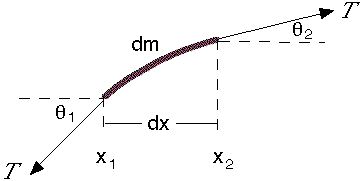
\includegraphics[width=0.3\textwidth]{figs/fig2.png} 
  \caption{Tensions acting on the small element of the string}
  \label{fig:2}
\end{figure}




 
The angle $\theta$ between the string and the $x$-direction is much smaller than 1, so $\sin \theta \approx \theta$ and $\cos \theta \approx 1$.
Let's apply Newton's second law in the vertical $y$ direction:
\begin{align}
F_y = ma_y
\end{align}

\begin{figure}[htb]
	\centering
	

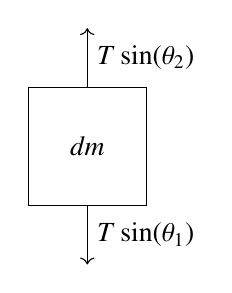
\begin{tikzpicture}[scale=0.75] % Adjust the scale factor as needed
    % Draw the square body
    \draw (0,0) rectangle node[pos=0.5] {$dm$} (2,2);
    
    % Add upward force T*sin(theta2)
    \draw[->, black] (1,2) -- node[right] {$T \sin(\theta_2)$} (1,3);
    
    % Add downward force T*sin(theta1)
    \draw[->, black] (1,0) -- node[right] {$T \sin(\theta_1)$} (1,-1);
\end{tikzpicture}




	\caption{Forces acting on the body in $Y$-direction}
	\label{fig:3}
\end{figure}

The sum of forces in the $Y$ direction is

From Figure~\figref{fig:2}
\begin{align}
F_y = T \sin \theta_2 - T \sin \theta_1 
\end{align}
Using the small angle approximation, $\sin \theta \approx \tan \theta = \frac{\partial y}{\partial x}$. So we may write:
\begin{align}
 F = T\left(\frac{dy}{dx}\Big|_2 - \frac{dy}{dx}\Big|_1\right) 
\end{align}
The acceleration in the $y$ direction is the rate of change in the $y$ velocity, so $a_y = \frac{\partial v_y}{\partial t} = \frac{\partial^2 y}{\partial t^2}$.Now,Newton’s second law in the $y$ direction
\begin{align}
 F = T\left(\frac{dy}{dx}\Big|_2 - \frac{dy}{dx}\Big|_1\right) = \mu dx \frac{d^2y}{dt^2} 
\end{align}
\begin{align}
 \frac{d^2y}{dt^2} = \frac{T}{\mu} \left(\frac{dy}{dx}\Big|_2 - \frac{dy}{dx}\Big|_1\right) 
\end{align}
Now we have been using the subscript 1 to identify the position $x$, and 2 to identify the position $(x+dx)$.
 
\begin{align}
 \frac{d^2y}{dt^2} = \frac{T}{\mu} \frac{d^2y}{dx^2} 
\end{align}
So the acceleration is proportional to the tension $T$ and inversely proportional to the mass per unit length $\mu$. 
It is also proportional to $\frac{\partial^2y}{\partial x^2}$.  $y = A \sin(kx - \omega t)$, Wave speed in a stretched string.

 However, to be a solution to 
\begin{align}
 \frac{d^2y}{dt^2} = \frac{T}{\mu} \frac{d^2y}{dx^2}, 
\end{align}
The second partial derivatives of $y = A\sin(kx - \omega t)$ with respect to $x$ and $t$ are given by:
\begin{align}
\frac{\partial^2 y}{\partial x^2} &= -k^2 A \sin(kx - \omega t), \\
\frac{\partial^2 y}{\partial t^2} &= -\omega^2 A \sin(kx - \omega t).
\end{align} In other words, $y = A \sin(kx - \omega t)$ is a solution provided that
\begin{align}
 \frac{T}{\mu} = \frac{\omega^2}{k^2}. 
\end{align}
In Travelling waves II, we saw that $\frac{\omega}{k}$ was the wave speed $v$, so we now have an expression for the speed of a wave in a stretched string:
\begin{align}
 v = \sqrt{\frac{T}{\mu}} 
\end{align}

This completes the derivation of the wave speed using first principles.

\textbf{1. Find the wavelength (\(\lambda\)) for the fundamental mode:}
\begin{equation}\label{eq:wavelength}
    \lambda = 2L \quad \Rightarrow \quad \lambda = 2 \times 0.875 \, \text{m} = 1.75 \, \text{m}
\end{equation}

\textbf{2. Use the frequency and wavelength to find the wave speed (\(v\)):}
\begin{equation}\label{eq:wavespeed}
    v = f \cdot \lambda \quad \Rightarrow \quad v = 45 \, \text{Hz} \times 1.75 \, \text{m} = 78.75 \, \text{m/s}
\end{equation}


\textbf{3. Use the wave speed (\(v\)) to find the tension (\(T\)) using the wave equation:}
\begin{equation}\label{eq:tension}
    T = \mu \cdot v^2 \quad  
    \end{equation}
    
\begin{equation}
\quad T = (4 \times 10^{-2} \, \text{kg/m}) \times (78.75 \, \text{m/s})^2 = 123.1875 \, \text{N}
\end{equation}

Therefore, the speed of the transverse wave on the string is $78.75 \, \text{m/s}$, and the tension in the string is $123.1875 \, \text{N}$.


\end{document}
